%\documentclass[10pt,handout]{beamer}

\documentclass[10pt]{beamer}
\usepackage[english]{babel} % Anpassa efter svenska. Ger svensk logga.
\usepackage[utf8]{inputenc} % Anpassa efter linux
\usepackage{graphicx}
\usepackage{hyperref}
\usepackage{listings}
%\input{../common/lststan} % Stan listing
\usepackage{lstbayes}
\usepackage[all,poly,ps,color]{xy}


\hypersetup{
    colorlinks=true,
    linkcolor=blue,
    filecolor=magenta,
    urlcolor=cyan,
}
\usepackage{../common/beamerthemeUppsala}
%\usetheme{Uppsala}
%\usecolortheme{UU} % Anpassa efter UU:s frger och logga
%\hypersetup{pdfpagemode=FullScreen} % Adobe Reader ska ppna fullskrm
\setbeamertemplate{itemize items}[circle]

% \usepackage{beamerthemesplit}
\usepackage{amsmath,amsfonts,amssymb}
% \usepackage{amssymb}
% \usepackage{graphics}
% \usepackage{graphicx}
% \usepackage{epsfig}
% \usepackage[latin1]{inputenc}
 \usepackage{color}
% \usepackage{fancybox}
% \usepackage{psfrag}
% \usepackage[english]{babel}
\usepackage{apacite}
\usepackage{bbm}
 \setbeamertemplate{footline}{\hfill\insertframenumber/\inserttotalframenumber}

% Input new commands
\input{../common/commands.tex}

\def\dashxy(#1){%
  /xydash{[#1] 0 setdash}def}
\def\grayxy(#1){%
  /xycolor{#1 setgray}def}
\newgraphescape{D}[1]{!{\ar @*{[!\dashxy(2 2)]} "#1"}}
\newgraphescape{P}[1]{!{\ar "#1"}}
\newgraphescape{F}[1]{!{*+=<2em>[F=]{#1}="#1"}}
\newgraphescape{O}[1]{!{*+=<2em>[F]{#1}="#1"}}
\newgraphescape{V}[1]{!{*+=<2em>[o][F]{#1}="#1"}}
\newgraphescape{B}[3]{!{{ "#1"*+#3\frm{} }.{ "#2"*+#3\frm{} } *+[F:!\grayxy(0.75)]\frm{}}}

%%%%%%%%%%%%%%%%%%%%%%%%%%%%%%%%%%%%%%%%%%%%%%%%%%%%%%%%%%%%%%%%%%

\setlength{\parskip}{3mm}
\title[]{{\color{black}Guest lecture: \\MCMC with Discrete Parameters}}
\author[]{Jakob Torgander}
\date{}

\begin{document}

\frame{\titlepage
% \thispagestyle{empty}
}

%%%%%%%%%%%%%%%%%%%%%%%%%%%%%%%%%%%%%%%%%%%%%%%%%%%%%%%%%%%%%%%%%%

\begin{frame}
	\frametitle{Outline}
		\begin{enumerate}
			\item Discrete parameters - Introduction \& discussion
			\item Describe three methods for computing posteriors with discrete latent parameters
			\begin{itemize}
				\item Marginalization
				\item Gibbs sampling
				\item Continuous approximation using Gumbel-Softmax-distribution
			\end{itemize}
			\item (Short) demonstration of methods.
		\end{enumerate}
\end{frame}

%%%%%% Section I %%%%%%%
\section{Discrete parameter models}

\begin{frame}
	\frametitle{Motivation}
	\begin{itemize}
		\item Discrete variables are everywhere
		\begin{itemize}
		 	\item Count data: e.g.\ number of car accidents
		 	\item Categorical data 
 			\item Decision/classification problems: (eg.\ yes/no)
 			\item Factor analysis
	 	\end{itemize}
		\item In many problems latent (hidden) discrete variables exists: conclusions changes if data is segmented into groups
		\item While current state-of-the-art method Hamiltonian Monte Carlo (HMC) works for discrete \textit{data} \uured{HMC does not directly work for discrete \textit{parameters}}.
		\end{itemize}
\end{frame}

\begin{frame}
	\frametitle{Case study - Gaussian mixture model} 
	\centering
	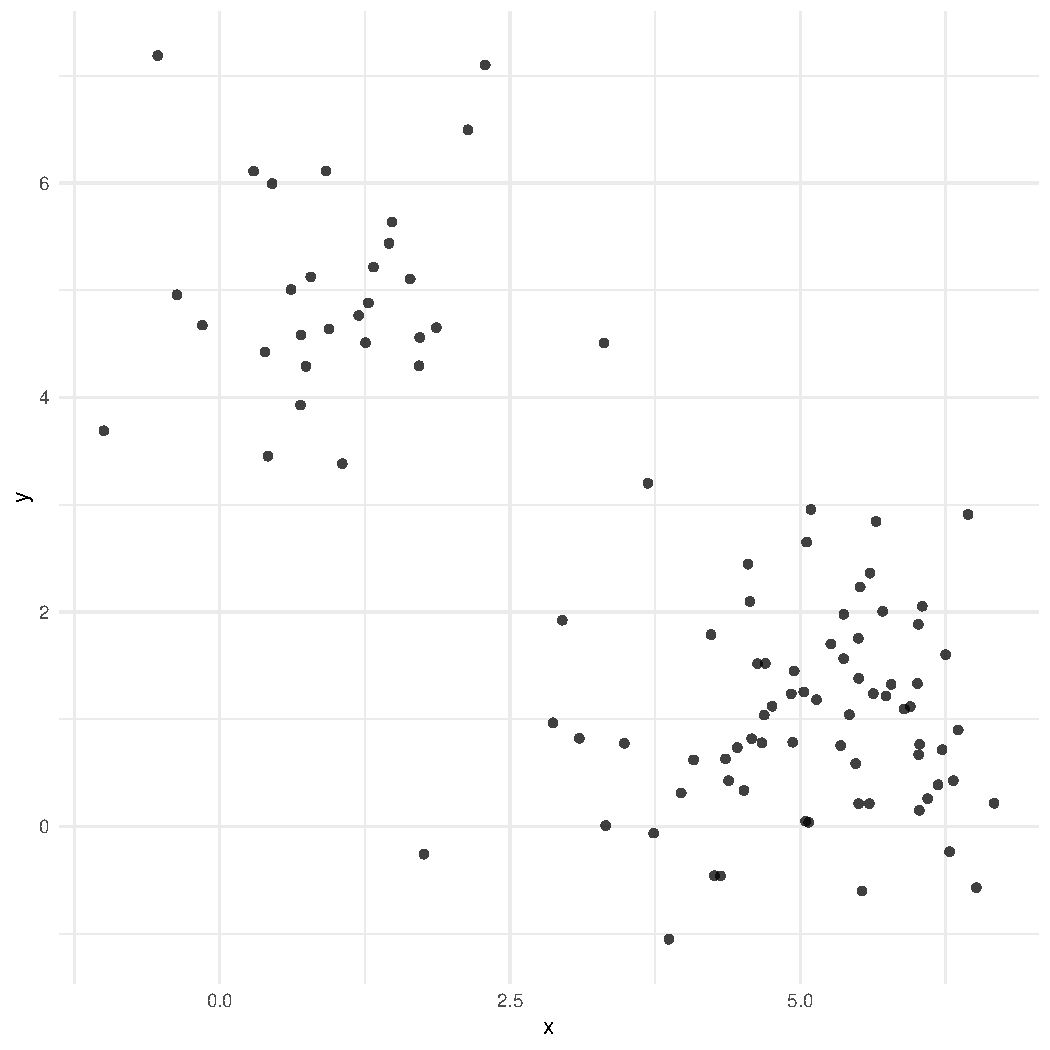
\includegraphics[width=6cm]{figs/data.pdf}
	\begin{itemize}
		\item Latent class variable $C$
		\item p(y) =$ \sum_{k = 1}^K \mathbbm{1}(C = k)\mathcal{N}(y | \mu_k, \sigma_k),$
		\item Task: identify cluster assignments, probabilities and centers
	\end{itemize}
\end{frame}

%%%%%% Section II %%%%%%
\section{Computation}

\frame{\sectionpage}
\begin{frame}
	\frametitle{Hamiltonian Monte Carlo (HMC) - Recap}
	\begin{figure}
		\centering
		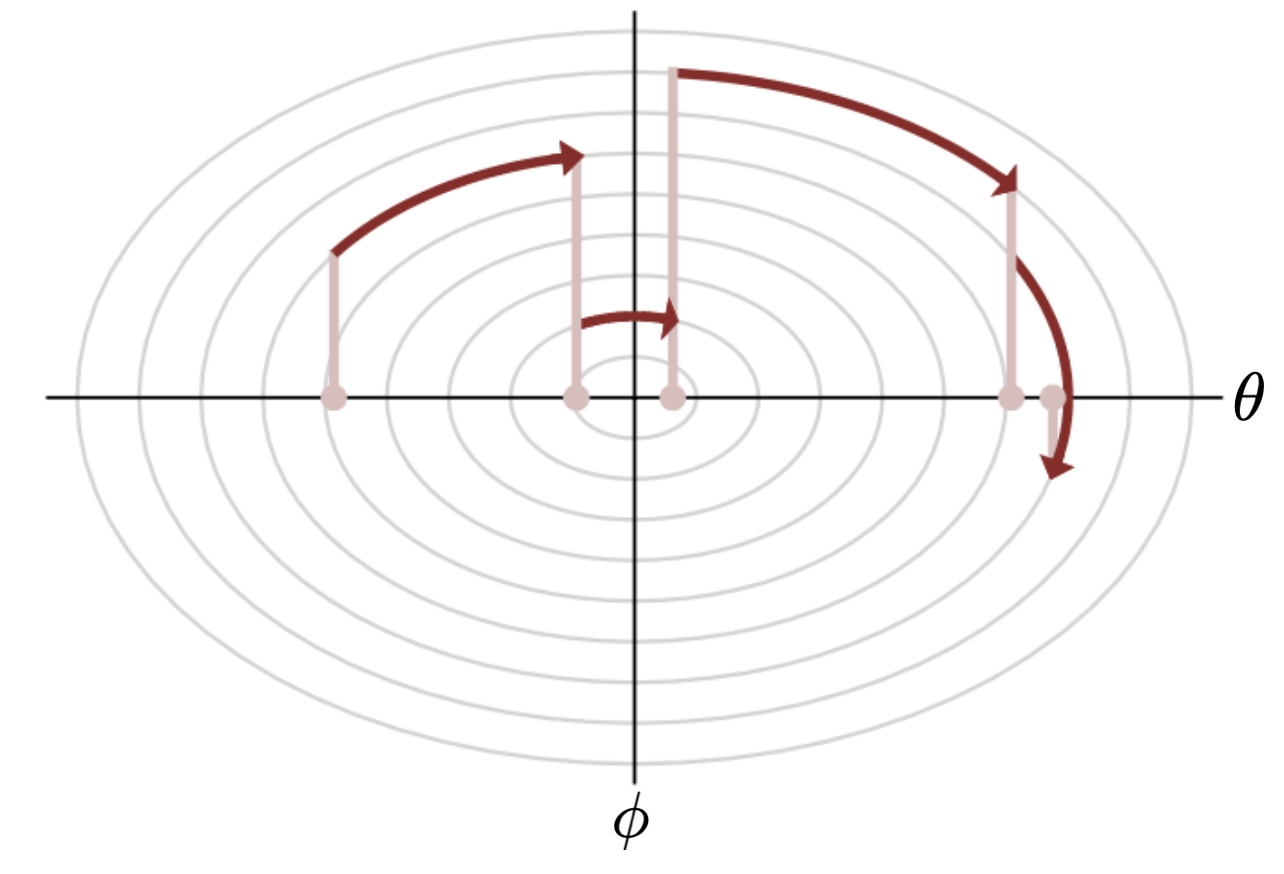
\includegraphics[width=5.5cm]{figs/hmc.png}
	\end{figure}
	\cite{betancourt}: Given a current parameter-momentum pair  $(\theta_i, \phi_i)$, Hamiltonian $H$ and mass matrix $M$:
	\begin{enumerate}
		\item Sample a new momentum variable $\phi_{i+1} \sim \mathcal{N}(0, M)$
		\item Lift $\theta_i$ onto the joint phase space $(\theta, \phi)$
		\item Integrate the flow defined by $H(\theta_i, \phi_{i+1}) =$ constant using Hamilton's equations
		\item Project back to original parameter space to receive new parameter sample $\theta_{i+1}$
	\end{enumerate}
\end{frame}

\begin{frame}
	\frametitle{Recap: the leapfrog integrator}
Step \uured{3} of HMC is based on the leapfrog algorithm
	\begin{align*}
		\psi \leftarrow &\psi + \frac{1}{2}\epsilon \frac{d\log q(\theta|y)}{d\theta} && \textcolor{blue}{1st\,momentum\, update}\\
		\theta \leftarrow& \theta + \epsilon M^{-1}\psi  && \textcolor{blue}{Parameter\,update}\\
		\psi \leftarrow &\psi  + \frac{1}{2}\epsilon \frac{d\log q(\theta|y)}{d\theta} && \textcolor{blue}{2nd \,momentum\, update},
	\end{align*}
	where $q$ denotes the target posterior density.\pause 
	\centering
	\textcolor{red}{Q: Why does this fail when q is discrete?}
\end{frame}

\begin{frame}
	\frametitle{HMC does not work for discrete posteriors}
	Main problem:
	Computation of the gradient  $\frac{d\log q(\theta|y)}{d\theta}$ requires the limits (partial derivatives)
	\begin{equation*}
		\frac{\partial q}{\partial \theta_i} = \lim_{h\to 0} \frac{q(\theta+h\boldsymbol{e}_i) - q(\theta)}{h}
	\end{equation*}
	to exist. This only happens when $q$ is continuous!
	\end{frame}
	
\subsection{Method  1: Marginalization}

\begin{frame}
	\frametitle{Method  1: Marginalization}
	Idea: Sum (marginalize) out the latent discrete parameters \cite{stan}. \\
	By the law of total probability:
	\begin{equation*}
		p(y) = \sum_{k= 1}^K p(y|c_k)p(c_k).
	\end{equation*}
	Then, $p(y)$ is continuous if $p(y|c_k), p(c_k)$ are. 
 \end{frame}
 
\begin{frame}
	 \frametitle{Marginalization}
 	\uured{Example:} for the GM-model:
	\begin{equation*}
		p_Y(y, |\pi, \mu, \sigma) = \sum_{k=1}^K\underbrace{\pi_k}_{\uured{p(c_k)}}\underbrace{\mathcal{N}(y | \mu_k, \sigma_k)}_{\uured{p(y|c_k)}},
	\end{equation*}
	where $\pi_k$ are (continuous) parameters.\pause
	\uured{Remark:} Compare with the original model formulation
	\begin{equation*}
		p(y|\pi, \mu, \sigma) = \sum_{k = 1}^K \mathbbm{1}(C = k)\mathcal{N}(y | \mu_k, \sigma_k)
	\end{equation*}
\end{frame}

\subsection{Method  2: Gibbs sampling}

\begin{frame}
	\frametitle{Method 2: Gibbs sampling}
	\uured{Recall:} Gibbs sampling: conditional (or block) sampling of $\theta$
	\begin{equation*}
		\theta_j \sim p(\theta_j|\theta_{-j}, y)\pause
	\end{equation*}
	For the GM-model, with $\sigma$ known:
	\begin{enumerate}
		\item For each observation $y$, sample classes $c_i$ with probability 
		\begin{equation*}
			p(c_i | \mu, \sigma, y) = \frac{p(y| c_i )p(c_i)}{\sum_{j=1}^Kp(y | c_j)p(c_j)} = \frac{p(c_i)\mathcal{N}(y | \mu_i, \sigma)}{\sum_{j=1}^Kp(c_j)\mathcal{N}(y | \mu_j, \sigma)}
		\end{equation*}\pause
		\item Sample means $\mu_i$ using the conditional distributions $p(\mu_i | y, c_i)$ (normal if likelihood and prior for $\mu$ is  )
	\end{enumerate}	
\end{frame}

\subsection{Method 3: Continuous approximation (Gumbel-Softmax)}

\begin{frame}
	\frametitle{Method 3: Continuous approximation Gumbel-Softmax}
	\uured{Ideas:}
	\begin{itemize}
		\item Approximate a discrete (categorical) distribution with a continuous distribution.
		\item The approximated distribution can then be used with HMC
		\item Use the "Gumbel trick" \cite{gs} from the field of deep learning
	\end{itemize}
\end{frame}

\begin{frame}
	\frametitle{"The Gumbel trick"}
	\uured{Proposition:}  Let Z be a categorical r.w with probability distribution $\pi = (\pi_1,\dots, \pi_K)$ and let $G_i $ be Gumbel(0,1)-		distributed with density
	\begin{equation*}
		f_{G_i} = e^{-x-e^{-x}}.
	\end{equation*}
	Then the random variable
	\begin{equation*} 
		U = \arg\max_i G_i + \log \pi_i,
	\end{equation*}
	follows the same distribution as $Z$.\pause
	\textcolor{red}{Q: How to use the argmax-function in a density?}  
\end{frame}

\begin{frame}
	\frametitle{Gumbel-Softmax distribution}
	Idea by \citeA{gs}: Approximate argmax with the softmax function. 
	\begin{equation*}
		Y_i = \frac{\exp((\log(\pi_i) + G_i)/\tau)}{\sum_{j=1}^k\exp((\log(\pi_j) + G_j)/\tau)},
	\end{equation*}
	where $G_i$ are  Gumbel(0,1)-distributed and $\tau$ is a "temperature" parameter.\pause

	As $\tau$ approaches 0, $Y = (Y_1, \dots , Y_K)$ then tends to a "one-hot" vector on the form
	\begin{equation*}
		[0, \dots, 0, 1, 0, \dots,0 ],
	\end{equation*}	
	where a "1" in position $m$ indicates the $m$-th class.
\end{frame}

\begin{frame}
	\frametitle{Gumbel-Softmax distribution}
	This yields the Gumbel-Softmax (GS) density function:
	\begin{equation*}
		p_{\pi,\tau}(y_1,\dots, y_K) = (K-1)!\cdot\tau^{K-1}\Big(\sum_{i=1}^K\pi_i/y_i^\tau\Big)^{-k}\prod(\pi_i/y_i^{\tau+1}). 
	\end{equation*}
	\textcolor{blue}{Continuous! Can hence be used with HMC and Stan.}
\end{frame}

\begin{frame}
	\frametitle{Methods - Summary}
	\begin{center}
	\resizebox{9.6cm}{!}{
		\begin{tabular}{ |c| c|   c|}
			\hline
			\textbf{Method}& \textbf{Pros} & \textbf{Cons}\\ 
			 \hline
			Marginalization  &  Works efficiently  & Does not return\\  
			& with HMC& the discrete parameter\\
			\hline
			 Gibbs & Returns classes, & Difficult (\& sometimes less efficient)   \\
 			& reliable for "simple" distributions & for non-conjugate distributions  \\
			\hline
			Gumbel-Softmax. & Returns classes, & High dependency on temperature $\tau$, \\
 			& works with HMC &  leapfrog (very) unstable for low temperatures  \\
			 \hline
		\end{tabular}
		}
	\end{center}
\end{frame}

%%%%%% Section III %%%%%%

\section{Demonstration}
\frame{\sectionpage}

\begin{frame}
	\centering
	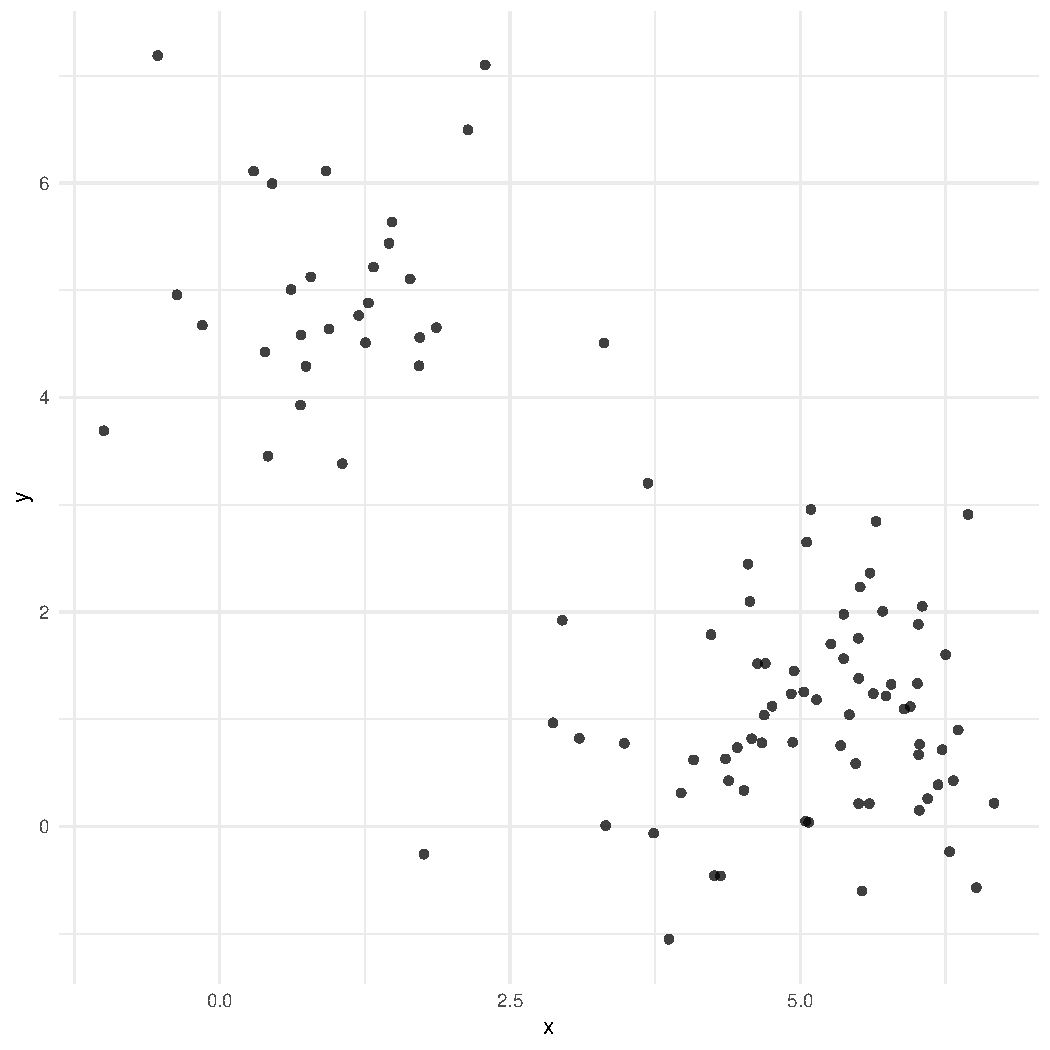
\includegraphics[width=4cm]{figs/data.pdf}
	\begin{itemize}
		\item Data: simulated gaussian mixtures with means $\mu_1 = (1,5), \mu_2 = (5,1)$ and $\sigma_1 = \sigma_2 = \mathbf{I}$
		\item Weakly informative $\mathcal{N}(0, 10)$-prior used for all $\mu$
		\item Dirichlet(1,1)-prior (see e.g. \cite[p.~69]{bda}) used for HMC methods (1 and 3)
		\item 2000 samples generated for each method
	\end{itemize}
\end{frame}

\begin{frame}
	\centering
	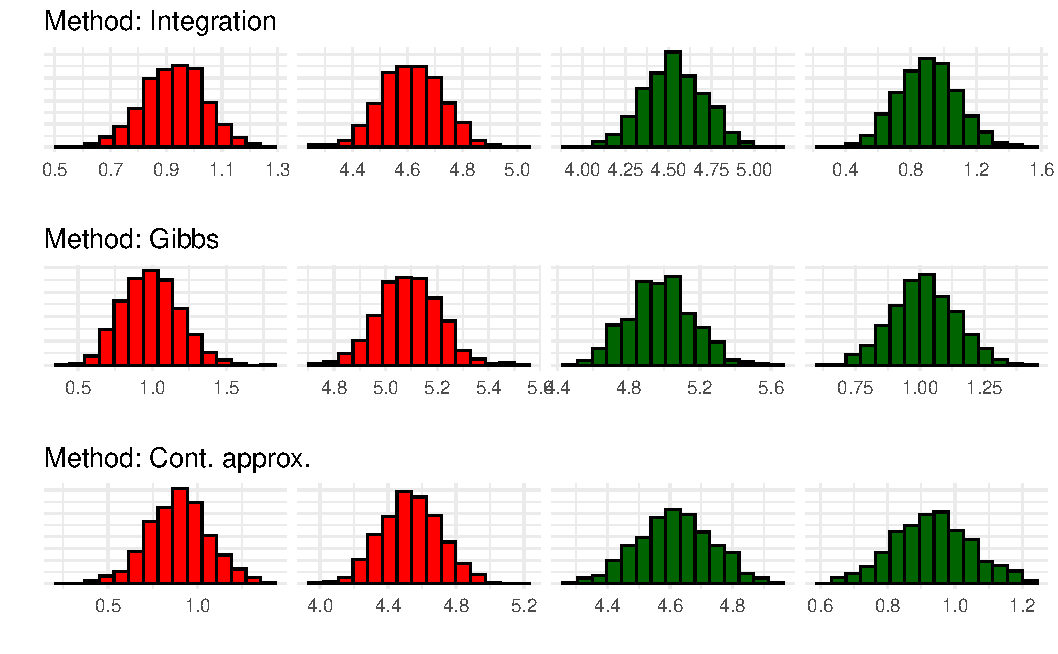
\includegraphics[width=9cm]{figs/means.pdf}
	\begin{itemize}
		\item All three methods correctly identify the centers\\ (red = $\mu_1$, green = $\mu_2$)
		\item Gibbs sampler closer to "ground truth" in this case
		\item Difference possible due to weakly informative Dirichlet prior of Method 1,3. Needs further investigation..
	\end{itemize}
\end{frame}

\begin{frame}
	\centering
	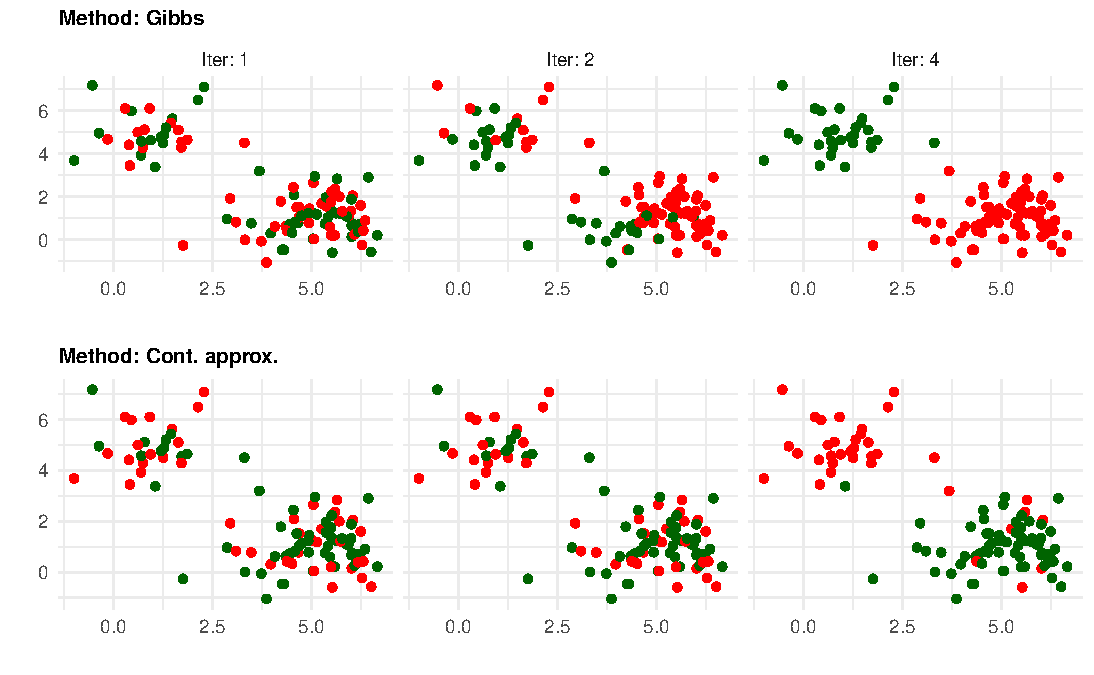
\includegraphics[width=9cm]{figs/iters.pdf}
	\frametitle{Class assignments - convergence}
	\begin{itemize}
		\item Both Gibbs and Continuous approx. converges quickly to the correct classes
		\item Gibbs sampler one iteration quicker
		\end{itemize}
	\end{frame}

\begin{frame}
	\frametitle{Use case: imputing missing values}
	\centering
	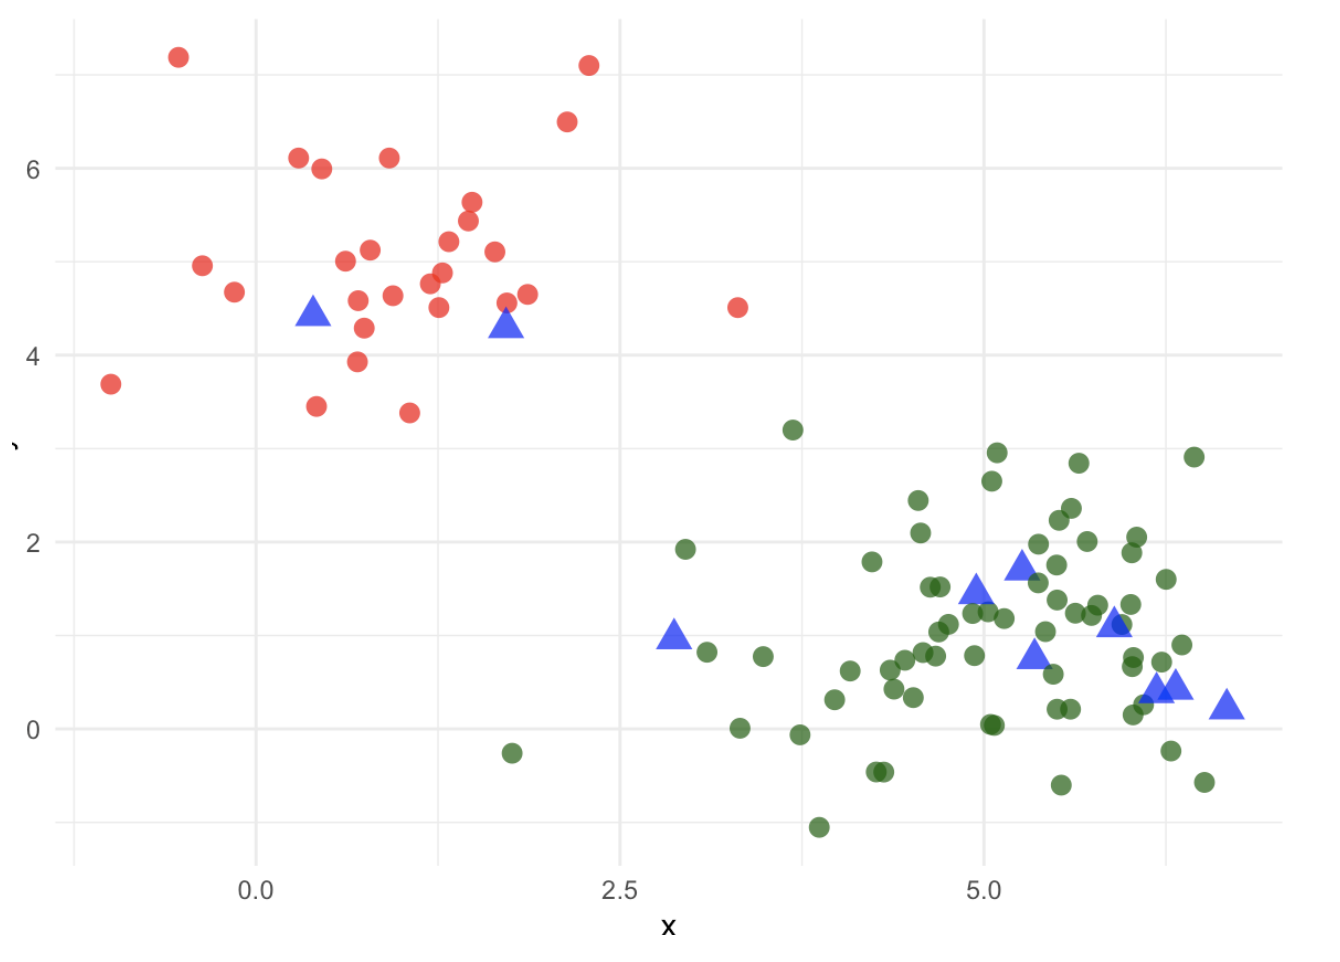
\includegraphics[width=4.6cm]{figs/preimpute.png}
	$\to$
	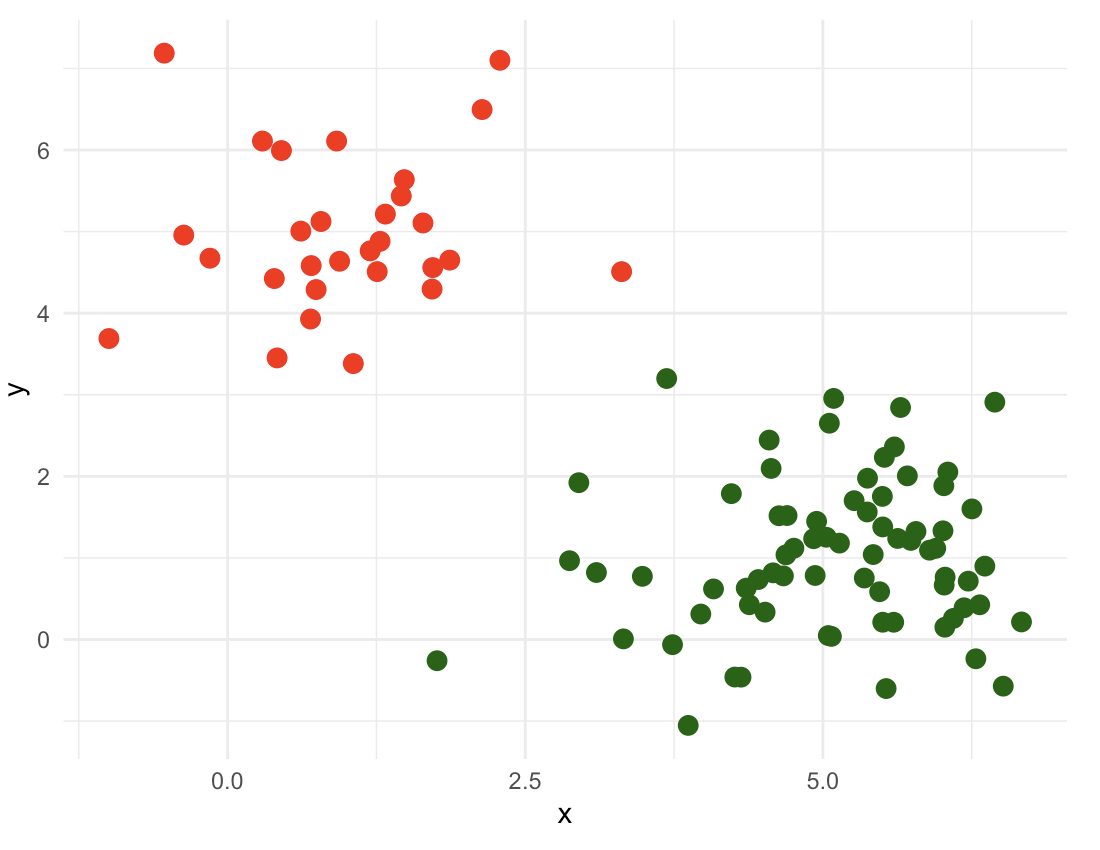
\includegraphics[width=4.1cm]{figs/postimpute.png}
	\begin{itemize}
		\item Gibbs, and Gumbel-Softmax method can be used to impute missing values (classes)
		\item Idea: Generate class parameter if  non-present in the data and use the actual class otherwise
		\item For general tips about handling missing values, see \cite{stanmissing}
	\end{itemize}
\end{frame}

\begin{frame}
	\frametitle{Future research}
	\begin{itemize}
		\item How do the methods scale with data size and dimension?
		\item How can $\tau$ in the GS-approximation be selected and tuned?
		\item Performance and convergence of methods on more complicated, high-dimensional posteriors?
	\end{itemize}
\end{frame}

\begin{frame}
	\centering
	Thank you!
	\end{frame}

%%%%%% References %%%%%%
\begin{frame}
	\frametitle{References}
	\bibliographystyle{apacite}
	\bibliography{MCMCDiscreteParams}
\end{frame}

%%%%%%%%%%%%%%%%%%%%%%%%%%%%%%%%%%%%%%%%%%%%%%%%%%%%%%%%%%%%%%%%%%


\end{document}
